\documentclass[a4paper,14pt]{extarticle}

\usepackage[top=1in, bottom=1in, left=1in, right=1in]{geometry}
\usepackage[utf8]{inputenc}
\usepackage[russian]{babel}
\usepackage{graphicx}
\usepackage{caption}
\usepackage{subcaption}
\usepackage{chngcntr}
\usepackage{amsmath}
\usepackage{amsfonts}
\usepackage{pgfplots}
\usepackage{pgfplotstable}
\usepgfplotslibrary{fillbetween}
\usepackage{float}
\usepackage{lipsum}% http://ctan.org/pkg/lipsum
\usepackage{multicol}% http://ctan.org/pkg/multicol
\usepackage{hhline}
\usepackage{tabularx}
\usepackage{tikz,xcolor}
\usepackage{tkz-graph}
\usepackage{float}
\usepackage{mathtools}
\usepackage{todonotes}
\usepackage{listings}
\usepackage[makeroom]{cancel}

\usetikzlibrary{arrows, petri, topaths}

\counterwithin{figure}{section}
\counterwithin{equation}{section}
\counterwithin{table}{section}

\begin{document}
\begin{titlepage}
\centering 
{\bfseries Санкт-Петербургский Политехнический Университет} \\
Институт компьютерных наук и технологий \\
Кафедра компьютерных систем и программных технологий \\
\vspace{5cm}
{\centering \textbf{Отчёт о лабораторной работе 8} \\ 
\vspace{0.2cm}
\textbf{Дисциплина}: Телекоммуникационные технологии \\
\vspace{0.2cm}
\textbf{Тема}: Модель телекоммуникационного канала. } \\
\vspace{4cm}
\hfill {\bfseries Работу выполнил:}  \\
\hfill гр. 33501/2 Вахаев И.Н. \\
\hfill {\bfseries Преподаватель}  \\
\hfill Богач Н.В.
\vfill
Санкт-Петербург \\
{\large 2018}
\end{titlepage}

\section{Цель работы}
Пакетный сигнал длительностью 200 мкс состоит из 64 бит полезной информации и 8 нулевых tail-бит. В нулевом 16-битном слове пакета передается ID, в первом - период излучения в мс, во втором – сквозной номер пакета, в третьем - контрольная сумма (CRC-16). На передающей стороне пакет сформированный таким образом проходит следующие этапы обработки: 

1. Помехоустойчивое кодирование сверточным кодом с образующими полиномами 753, 561( octal ) и кодовым ограничением 9. На выходе кодера количество бит становится равным 144. 

2. Перемежение бит. Количество бит на этом этапе остается неизменным. 

3. Модуляция символов. На этом этапе пакет из 144 полученных с выхода перемежителя бит разбивается на 24 символа из 6 бит. Генерируется таблица функций Уолша длиной 64 бита. Каждый 6- битный символ заменяется последовательностью Уолша, номер которой равен значению данных 6-ти бит. Т.о. на выходе модулятора получается 24 * 64 = 1536 знаковых символов. 

4. Прямое расширение спектра. Полученная последовательность из 1536 символов периодически умножается с учетом знака на ПСП длиной 511 символов. Далее к началу сформированного символьного пакета прикрепляется немодулированная ПСП. Т.о. символьная длина становится равной 1747. Далее полученные символы модулируются методом BPSK . Задача: по имеющейся записи сигнала из эфира и коду модели передатчика создать модель приемника, в которой найти позицию начала пакета и, выполнив операции демодуляции, деперемежения и декодирования, получить передаваемые параметры: ID, период, и номер пакета. Известно, что ID = 4, период 100 мс, номер пакета 373. Запись сделана с передискретизацией 2, т.е. одному BPSK символу соответствуют 2 лежащих друг за другом отсчета в файле. Запись сделана на нулевой частоте и представляет из себя последовательность 32-х битных комплексных отсчетов, где младшие 16 бит вещественная часть, старшие 16 бит – мнимая часть. Ниже приведена таблица перемежения и последовательность ПСП.

Основной задача - по имеющейся записи сигнала из эфира и коду модели передатчика создать модель приемника, в которой найти позицию начала пакета и, выполнив операции демодуляции, деперемежения и декодирования, получить передаваемые параметры: ID, период, и номер пакета.
Известно, что ID = 4, период 100 мс, номер пакета 373. Запись сделана с передискретизацией 2, т.е. одному BPSK символу соответствуют 2 лежащих друг за другом отсчета в файле. Запись сделана на нулевой частоте и представляет из себя последовательность 32-х битных комплексных отсчетов, где младшие 16 бит вещественная часть, старшие 16 бит – мнимая часть. 

\section{Теоретическая информация}
\subsection{Приём и передача сигналов}

Приёмник и передающее устройство выполняют последовательность операций над пакетом обмена данными. В канале передачи информации действуют шумы. Синхронизация записи сигнала по известной опорной псевдослучайной последовательности выполняется при неизвестных параметрах шума на приемнике. При демодуляции и одновременном сужении спектра принятого сигнала используется корреляционный метод. В обоих случаях - при синхронизации и при сужении спектра определяется максимальный по значению элемент строки матрицы результатов, который указывает на начало пакета(при синхронизации) или на бинарный номер строки матрицы Уолша(при сужении спектра и демодуляции).

\section{Ход работы}

Была задана ПСП(псевдослучайная последовательность):

\begin{figure}[H]
\center{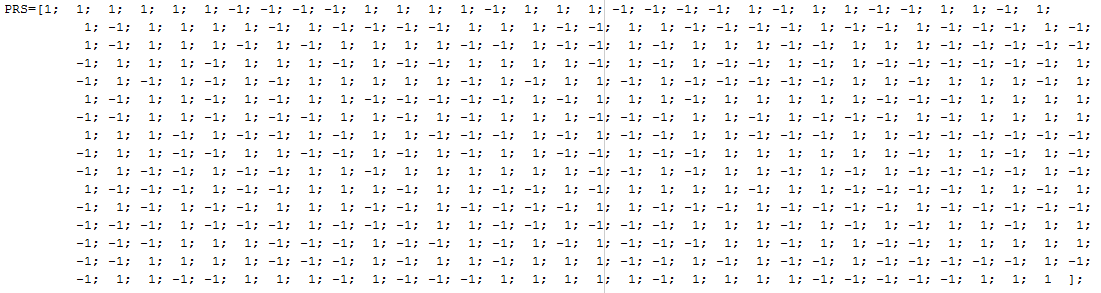
\includegraphics[width=1\linewidth]{screen/1}}
\caption{ПСП}
\label{1}
\end{figure}

Затем взята последовательность перемежения:

\begin{figure}[H]
\center{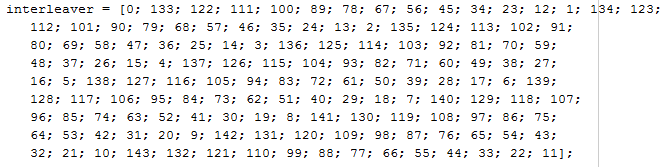
\includegraphics[width=1\linewidth]{screen/2}}
\caption{Последовательность перемножения}
\label{2}
\end{figure}

Получили сигнал (test.sig), который был создан с помощью transmittertract.m:

\begin{figure}[H]
\center{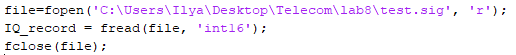
\includegraphics[width=1\linewidth]{screen/3}}
\caption{Чтение сигнала}
\label{3}
\end{figure}

Передискретизация равна 2, то есть отсчёты дублируются подряд.
Вещественная часть - нечётные числа, комплексная часть - чётные числа.
Были выделены реальная и мнимая части сигнала:

\begin{figure}[H]
\center{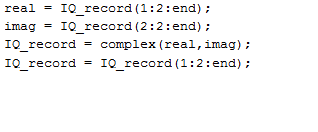
\includegraphics[width=1\linewidth]{screen/4}}
\caption{Выделение реальной и мнимой частей сигнала}
\label{4}
\end{figure}

Был демодулирован сигнал и построена матрица Уолша:

\begin{figure}[H]
\center{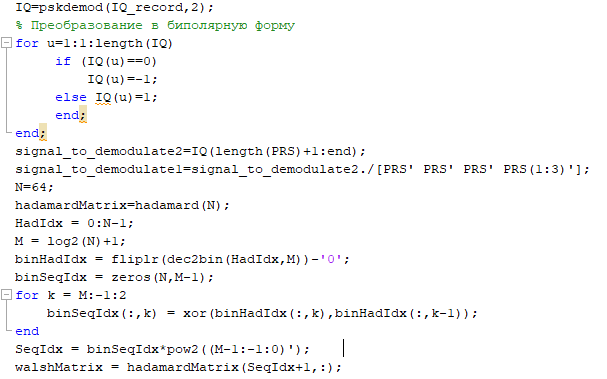
\includegraphics[width=1\linewidth]{screen/5}}
\caption{Код в Matlab}
\label{5}
\end{figure}

Перешли к двоичному виду:

\begin{figure}[H]
\center{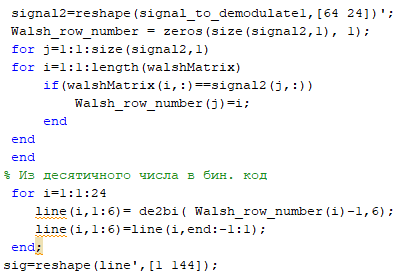
\includegraphics[width=1\linewidth]{screen/6}}
\caption{Код в Matlab}
\label{6}
\end{figure}

Произвели декодирование с учётом перемежения:

\begin{figure}[H]
\center{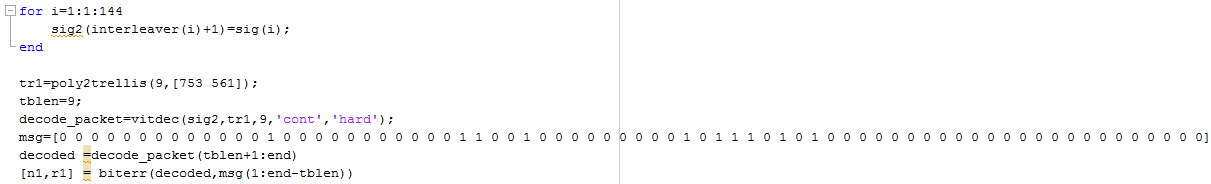
\includegraphics[width=1\linewidth]{screen/7}}
\caption{Код в Matlab}
\label{7}
\end{figure}

В декодированном пакете отсутствуют ошибки. Из этого следует, что задача была решена верно.


\section{Выводы.}

В данной работе мы создали модель приемника, выполняющую операции демодуляции, деперемежения и декодирования.

\end{document}
